\documentclass[
    11pt,
    a4paper,
    sfdefaults=false,
    toc=chapterentrywithdots,
    twoside,openright,
    titlepage,
    parskip=half,
    headings=normal,  % reduces heading size
    listof=totoc,
    bibliography=totoc,
    index=totoc,
    captions=tableheading,  % caption below table
    chapterprefix,
    listof=flat,
    final
]{scrbook}


% details about your thesis
\newcommand{\titel}{Gefahren im Metaverse: Social Engineering als Grundlage für Angriffe im Metaverse}
\newcommand{\artderarbeit}{Bachelorarbeit}  % {Bachelorarbeit,Masterarbeit}
\newcommand{\autor}{Andre Schindler}
\newcommand{\studiengang}{Wirtschaftsinformatik}  % {Informatik,Wirtschaftsinformatik,Medieninformatik}
\newcommand{\matrikelnr}{327\,2457}
\newcommand{\erstgutachter}{Prof.\,Dr.~Ronald Petrlic}
\newcommand{\zweitgutachter}{Prof.\,Dr.~Peter Rausch}
\newcommand{\betreuer}{M.Sc.\,~Martina Schmidt}
\newcommand{\unternehmen}{Musterfirma GmbH}
\newcommand{\logo}{figures/TH-Nuernberg-RGB.png}
\newcommand{\keywords}{hot, fuzz}
 

% custom head and foot
\usepackage[automark]{scrlayer-scrpage}
\pagestyle{scrheadings}
\ihead{\headmark}
\chead{}
\ohead{\pagemark}
\renewcommand*\chaptermarkformat{\chapappifchapterprefix{\ }% 
  \thechapter.\enskip}

\RedeclareSectionCommand[tocindent=0pt]{section}
\RedeclareSectionCommand[tocindent=0pt]{subsection}
%\RedeclareSectionCommand[tocnumwidth=70pt]{chapter}

\usepackage{scrhack}

% other packages
\usepackage[utf8]{inputenc}
\usepackage[T1]{fontenc}
\usepackage{lmodern,relsize,textcomp,csquotes}
\usepackage{amsmath,amsfonts}
\usepackage[ngerman]{babel}  % flip for German thesis
\usepackage[final]{graphicx}
\usepackage{setspace,geometry,xcolor}
\usepackage{makeidx}
\usepackage{paralist,ifthen,todonotes}
\usepackage{url}
\usepackage[toc]{glossaries}
\usepackage{pdfpages}

% table setup
\usepackage{longtable}
\usepackage{array}
\usepackage{ragged2e}
\usepackage{lscape}

% pdf hyperref
\usepackage[
    bookmarks=true,
    bookmarksopen=true,
    bookmarksnumbered=true,
    bookmarksopenlevel=1,
    pdftitle={\titel},
    pdfauthor={\autor},
    pdfcreator={\autor},
    pdfsubject={\titel},
    pdfkeywords={\keywords},
    pdfpagelabels=true,
    colorlinks=true,
    linkcolor=red,
    urlcolor=magenta,
    anchorcolor=black,
    citecolor=cyan,
    filecolor=magenta,
    menucolor=red,
    plainpages=false,
    hypertexnames=true,
    linktocpage=true,
]{hyperref}

% configure your listings style
\usepackage{listings}
\lstset{
	tabsize=3,
	extendedchars=true,
	frame=single,
	showstringspaces=true,
	numbers=left,
	numberstyle=\small,
	breakautoindent=true
}

% page setup
% \setlength{\topskip}{\ht\strutbox}
\geometry{paper=a4paper,left=2.5cm,top=3.0cm,bindingoffset=.8cm}
\onehalfspacing
\frenchspacing
\clubpenalty = 10000
\widowpenalty = 10000 
\displaywidowpenalty = 10000

% some commands
\newcommand{\ua}{\mbox{u.\,a.\ }}
\newcommand{\zB}{\mbox{z.\,B.\ }}
\newcommand{\dahe}{\mbox{d.\,h.,\ }}
\newcommand{\bzw}{\mbox{bzw.\ }}
\newcommand{\bzgl}{\mbox{bzgl.\ }}
\newcommand{\eg}{\mbox{e.\,g.\ }}
\newcommand{\ie}{\mbox{i.\,e.\ }}
\newcommand{\wrt}{\mbox{w.\,r.\,t.\ }}
\newcommand{\etal}{\mbox{\emph{et.\,al.\ }}}


% TODO remove if not needed...
\usepackage{blindtext}

% load glossary entries
\makenoidxglossaries
\loadglsentries{glossary}

\begin{document}

\setcounter{secnumdepth}{3}  % numerate subsections
\setcounter{tocdepth}{2}  % ...but don't include them in toc

\frontmatter
\include{cover}\cleardoublepage

% download the following form and complete it (hit save in your editor)
% https://intern.ohmportal.de/fileadmin/Gelenkte_Doks/Abt/SZS/SB/SB_0050_FO_Pruefungsrechtliche_Erklaerung_und_Erklaerung_zur_Veroeffentlichung_der_Abschlussarbeit_public.pdf
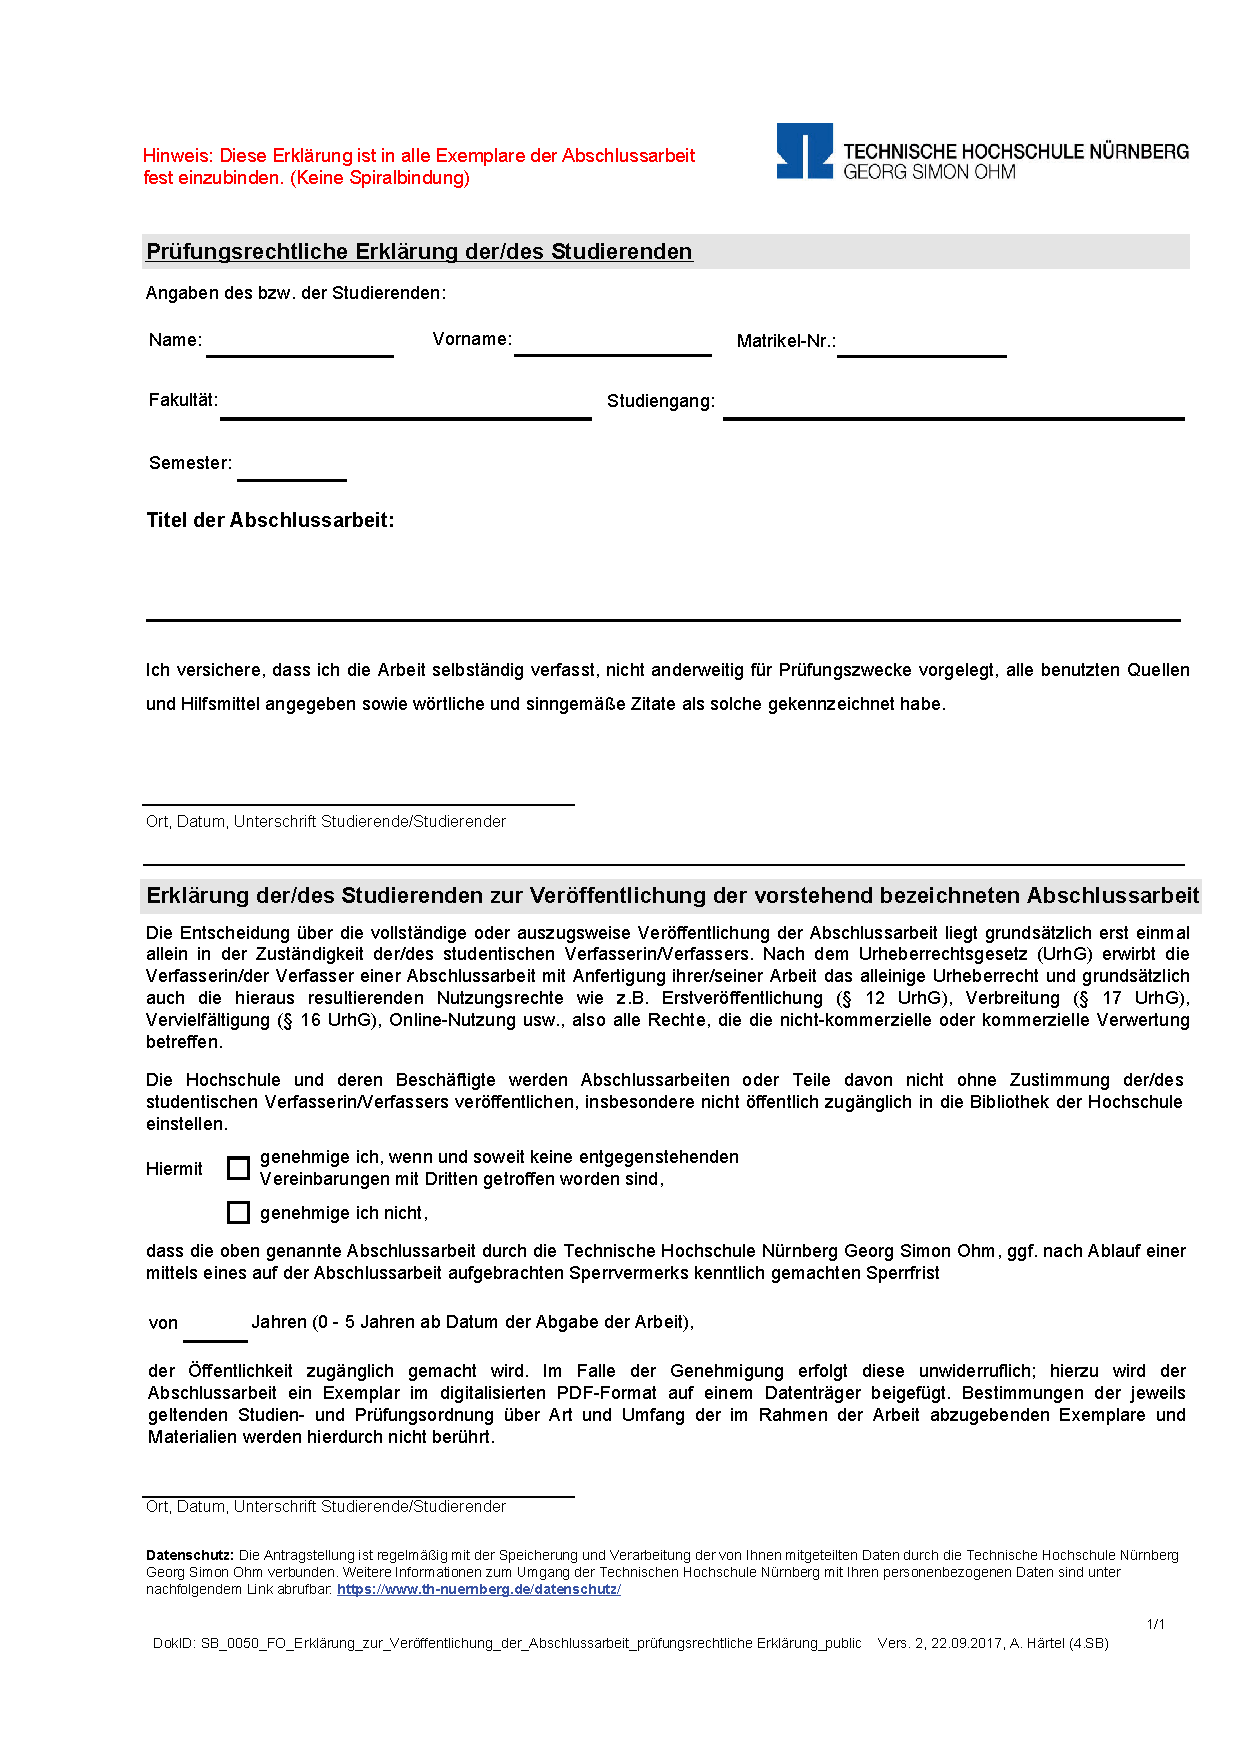
\includepdf{SB_0050_FO_Pruefungsrechtliche_Erklaerung_und_Erklaerung_zur_Veroeffentlichung_der_Abschlussarbeit_public.pdf}\cleardoublepage

\chapter{Anleitungen und Tests}\label{ch:Anleitungen}

\section{Anleitungen}
In this chapter, we're actually using some code!

%\begin{lstlisting}[language=Python,caption={This is an example of inline listing},captionpos=b]
%x = 1
%if x == 1:
%    # indented four spaces
%    print("x is 1.")

%\end{lstlisting}

%You can also include listings from a file directly:

%\lstinputlisting[language=Python,caption={This is an example of included listing},captionpos=b]{listings/example.py}




\subsection{And an even more important subsection}

It is possible to reference glossary entries as \gls{library} as an example.

\section*{Tests}


Definitionen Metaverse \cite{Ball22}
\\Definitionen Metaverse \cite{Drip22} \\
Seite 46 gegen wen Kämpfwn wir \cite{Hypp22}\\
Psychologie hinter SocialEngeneering \cite{schu11}\\
Kunst des Human Hacking \cite{Hadn11}



You can also write footnotes.\footnote{Footnotes will be positioned automatically.}

äüö


\thispagestyle{empty}
\section*{Kurzdarstellung}
\label{sec:kurzdarstellung}

\subsection{Was ist zu tun}
Kurze Zusammenfassung der Arbeit, höchstens halbe Seite.
Nenne die Zielsetzung, die Problemstellung und die Forschungsfragen. Wenn deiner Abschlussarbeit bestimmte Hypothesen zugrunde liegen, erwähne diese auch.
\\ \url{https://www.scribbr.de/aufbau-und-gliederung/abstract-schreiben/}


\subsection{Kurzdarstellung}
Das Ziel in der vorliegenden Arbeit ist es, zu klären, durch welche\dots


\cleardoublepage

\tableofcontents

\mainmatter
\chapter{Einleitung}\label{ch:Einleitung}



\chapter{Metaverse}\label{ch:Metaverse}

\section{Definitionen und Konzepte}
Definition des Metaversums: Diskutiere verschiedene Definitionen und Konzepte des Metaversums, um deinen Lesern ein Verständnis dafür zu vermitteln, was das Metaverse ist und wie es sich von anderen virtuellen Welten unterscheidet.


\subsection{verschiedene Definitionen}

\subsection{eigene Definition}

\section{Technologien}
Erkläre die verschiedenen Technologien, die im Metaverse eingesetzt werden, wie VR-Brillen, AR-Brillen, Digital Twins und KI, und diskutiere deren Potenzial für die Schaffung immersiver virtueller Erfahrungen.

\subsection{Virtuel Reality}
\subsection{Augmented Reality}
\subsection{Digitale Zwillinge}
\subsection{Künstliche Intiligenz}
\subsection{Kryptowährungen}




\chapter{Social Engineering}\label{ch:SocialEngineering}

\section{Definition}

%Köder Phishing etc
\section{Psychologie hinter Social Engineering}
\subsection{Reziprozität}
\subsection{Commitment und Konsistenz}
\subsection{Obedience to Authority}
\subsection{Sympathie}

\section{Ablauf eines Angriffs}
\chapter{Gefahren im Metaverse}\label{ch:GefahrenimMetaverse}

\section{Identitätsdibstahl}
TODO

Beispiel Warframe

\section{Biometrische Hacks}
TODO

Brillen können gehackt werden Biometrische Daten ausgelesen werden wie mimiken etc 

\section{Deep Fakes}
TODO

Avatar ist ein Gegenstand und kann lauschen

\chapter{Zusammenfassung}\label{ch:Zusammenfassung}


\chapter{Fazit und Ausblick}\label{ch:FazitundAusblick}

TODO

Sicherheit vorgegaukelt die so noch nicht vorhanden ist. Schwachstelle Mensch 





% remove if not needed
%\appendix
%\chapter{Supplemental Information}\label{app:supplemental-information}





\backmatter
\listoffigures
\cleardoublepage

\listoftables
\cleardoublepage

%\renewcommand{\lstlistlistingname}{List of Listings}  % change for German thesis
%\lstlistoflistings
%\cleardoublepage

\bibliographystyle{wmaainf}
\bibliography{refs}

\printnoidxglossaries

\end{document}
